\documentclass[a4paper,
fontsize=11pt,
%headings=small,
oneside,
numbers=noperiodatend,
parskip=half-,
bibliography=totoc,
final
]{scrartcl}

\usepackage{synttree}
\usepackage{graphicx}
\setkeys{Gin}{width=.6\textwidth} %default pics size

\graphicspath{{./plots/}}
\usepackage[ngerman]{babel}
%\usepackage{amsmath}
\usepackage[utf8x]{inputenc}
\usepackage [hyphens]{url}

\usepackage[colorlinks, linkcolor=black,citecolor=black, urlcolor=blue,
breaklinks= true]{hyperref}
\usepackage{booktabs} 
\usepackage[left=2.4cm,right=2.4cm,top=2.3cm,bottom=2cm,includeheadfoot]{geometry}
\usepackage{eurosym}
\usepackage{multirow}
\usepackage[ngerman]{varioref}
\setcapindent{1em}
\renewcommand{\labelitemi}{--}
\usepackage{paralist}
\usepackage{pdfpages}
\usepackage{lscape}
\usepackage{float}
\usepackage{acronym}
\usepackage{eurosym}
\usepackage[babel]{csquotes}
\usepackage{longtable,lscape}
\usepackage{mathpazo}
\usepackage[flushmargin,ragged]{footmisc} % left align footnote

\urlstyle{same}  % don't use monospace font for urls

\usepackage[fleqn]{amsmath}

%adjust fontsize for part

\usepackage{sectsty}
\partfont{\large}

%Das BibTeX-Zeichen mit \BibTeX setzen:
\def\symbol#1{\char #1\relax}
\def\bsl{{\tt\symbol{'134}}}
\def\BibTeX{{\rm B\kern-.05em{\sc i\kern-.025em b}\kern-.08em
    T\kern-.1667em\lower.7ex\hbox{E}\kern-.125emX}}

\usepackage{fancyhdr}
\fancyhf{}
\pagestyle{fancyplain}
\fancyhead[R]{\thepage}

%meta
%meta

\fancyhead[L]{Redaktion LIBREAS \\ %author
LIBREAS. Library Ideas, 24 (2014). % journal, issue, volume.
\href{http://nbn-resolving.de/urn:nbn:de:kobv:11-100215955}{urn:nbn:de:kobv:11-100215955}} % urn
\fancyhead[R]{\thepage} %page number
\fancyfoot[L] {\textit{Creative Commons BY 3.0}} %licence
\fancyfoot[R] {\textit{ISSN: 1860-7950}}

\title{\LARGE{Editorial LIBREAS \#24: Zukünfte}} %title %title
\author{Redaktion LIBREAS} %author

\date{}
\begin{document}

\maketitle
\thispagestyle{fancyplain} 

%abstracts

%body
\begin{quote}
\enquote{Future Librarians will find themselves working for a different
kind of organization than they have worked for in the past.} (John T.
Eastlick (1971): The Librarian's Environment. In: John T. Eastlick
(ed.): The Changing Environment of Libraries. Chicago: ALA, 1971, S.
73-77. S.76)
\end{quote}

Gemeinplätze und Zitate zur Zukunft von leidlich semantischer Relevanz
bis zum Taupunkt Tautologie sind in endloser Zahl vorhanden. Dies gilt
für nahezu alle Sprachen und alle Kulturen. Dass man sie im
Bibliothekswesen findet, überrascht daher nicht. Und wo sie in den
Diskurs eintauchen, folgen sie meist denselben Mustern: Die Relevanz der
Behauptung, Bibliotheken müssten zukunftsfähig sein, wird mit der
Behauptung gestützt, Bibliotheken seien so, wie sie jetzt sind, eher
nicht zukunftsfähig -- das aber in Abwandlungen. Denn die Welt da
draußen, die ihnen gesellschaftlicher, politischer, technologischer
Rahmen sind, erzwingt eine passende Reaktion der Bibliotheken auf ihren
eigenen Wandel. Wo die Bibliothek den Zwängen des Außen, ihrer Nutzer
und Nutzerinnen, der Zeit nicht folgt, wird ihr Gelände schnell sumpfig.
Eine Weile mag man sie noch sehen, aber früher oder später wird sie
untergehen.

Der Gegendiskurs ist gar kein wirklicher Gegendiskurs, denn niemand
behauptet, die Bibliotheken müssten so bleiben, wie sie immer waren. So
ein \enquote{Immer} gibt es nicht, jedenfalls nicht verbindlich,
höchstens in der Wahrnehmung dessen, der um sein persönliches
Bibliotheksideal streitet. Der Gegendiskurs ist einer der Relativierung.
Er traut der Bibliothek und den Bibliotheksakteuren ein wenig mehr zu.
Während die Fatalisten davon ausgehen, dass die Bibliotheken allein über
Anpassung an die bibliotheksexterne Welt überleben können, argumentieren
die Relativisten, dass die Bibliothek zur aktiven Eigenbeteiligung an
der Zukunft befähigt sei. In welchem Umfang, scheint hauptsächlich eine
Frage von Macht und Mut. Dass es aber in der Bibliotheksgeschichte immer
wieder Avantgardisten und Visionäre gab -- man denke nur an Akteure wie
Paul Otlet -- die ihrer Zeit mit ihren Ideen deutlich voraus waren,
schließt zumindest die Möglichkeit einer nachdrücklicheren Würdigung der
Mitgestaltungsthese nicht aus. Es ist eigentlich wie überall: Es kommt
gar nicht so sehr auf die Institution an und auch nicht auf den Inhalt,
sondern auf die einzelnen Akteure und Akteurinnen. Wenn die Bibliothek
gestaltend tätig sein möchte, muss sie attraktiv für die Gestaltenden
sein. Wenn man nicht die Arbeitsbedingungen des Googleplex oder eines
Apple Campus zu bieten hat, könnte man im Zeitalter nach Snowden
vielleicht auf die alten Werte der Aufklärung rekurrieren und damit
locken, dass das Bibliothekswesen von Parteilichkeit soweit entfernt
ist, wie von auf ästhetischen Idealen und Don't-be-evil-Hohlheiten
aufgesetzten Quasi-Glaubensgemeinschaften, man also in der Tradition
einer rationalen, hoch reflektierten, ethischen und auf Inklusion
gerichteten Arbeit an der Vermittlung von Wissen steht. Die Zukunft der
Bibliotheken könnte die Fortsetzung des Mutes, einen eigenen Verstand zu
benutzen, ein eigenes Gewissen und eine Prise Verantwortungsethik zu
haben, mit den jeweils zeitgemäßen sozialen, technischen und
intellektuellen Handlungsmöglichkeiten darstellen. Dieser ideelle Kern
des Bibliothekswesens wird erstaunlicherweise oft nur sichtbar
aktiviert, wenn man ein klangvolles Motto für eine Großveranstaltung
braucht. Abseits davon werden die politischen, sozialen und
kulturgestaltenden Potentiale der Bibliothek bestenfalls mit leiser
Stimme hervorgebracht, wogegen schmissige Architekturmodelle und banale
E-Ausleih-Ideen regelmäßig inszeniert werden. Kein Wunder, denn ersteres
lässt sich nur schwer ökonomisieren. Die Rhetorik nach dem \enquote{next
big thing}, wodurch in der Regel gesättigte Bedürfnisse durch neue
befriedigt werden, funktioniert hier nicht. Und schlimmer: Schwer
ökonomisierbare kulturelle Gewandtheit verliert innerhalb dieser
Argumentationsschleife an Stimmkraft und scheidet im Wettbewerb um
Aufmerksamkeit oft genug aus. Es ist vielleicht weniger die Zukunft an
sich, sondern der Diskurs des \enquote{darüber}, welcher sich ändern
muss und wird.

Aber natürlich: Die Zukunft. Immer wieder und widersprüchlich.
Unterschiedliche Positionen sind zweifellos eine wichtige Voraussetzung
für jede sinnvolle Diskussion. Zudem ist es vermutlich eine
kulturanthropologische Grundkonstante, dass man Debatten im
Generationenrhythmus mit Ähnlichkeiten bis in die Nuancen wiederholen
muss. Die Diskussionen um die Zukunft der Bibliotheken und die dabei
aktiven Positionen lassen sich über die Jahrzehnte immer wieder in der
bibliothekarischen Literatur finden. Es gibt Verschiebungen. Aber man
entdeckt auch erstaunlich viele Konstanten. Die Bibliotheken, die
gesellschaftlichen und technischen Entwicklungen waren in den 1990er
Jahren, in den 1970er Jahren, in den 1910er Jahren unterschiedlich; aber
der Bezug zur Zukunft, teilweise ängstlich, teilweise hoffnungsvoll,
fand sich immer wieder. Eine einfache Recherche zur Schlagwortkette
\enquote{Zukunft Bibliothek} im Metakatalog der Wahl zeigt diese weit
zurückreichende Tradition auf. Bibliotheken sind in einem beständigen
Wandel begriffen, nicht erst seit zehn oder zwanzig Jahren, sondern seit
weit längerer Zeit. Eigentlich sind sie es seit dem Aufkommen der / des
Bibliothekswesen/s. Viele der Utopien und Dystopien über Bibliotheken
traten und treten nicht ein, vieles kommt anders -- besser oder
schlechter -- als erwartet. Aber: Bibliotheken sind beständig im Wandel
und diskutieren dies ebenso beständig. Das ist ein gutes Zeichen, zeugt
es doch von Vitalität. Aus dieser ergeben sich letztlich auch die
Verschiebungen, die dafür sorgen, dass wir doch nicht mehr in jedem
Aspekt analog zu den Debatten der 1950er um die Zukunft streiten. Heute
wissen wir zum Beispiel, dass das Bellen für oder gegen eine
wissenschaftliche-technische Revolution völlig für die Katz war.
Irgendwann standen ein paar Computer in den Bibliotheken -- auch wenn
wir zugegebenermaßen nicht wissen, wie sie ohne diese
gesamtgesellschaftlichen Debatten ausgesehen hätten -- und die
unbestreitbaren Vorteile des OPACs im Raum. Jetzt können wir unsere
Fantasien auf deren Zukunft projizieren. Blicken wir auf die
Grabenkämpfe vergangener Zukunftsdiskurse zurück, erkennen wir auch, wie
müßig Halsstarrigkeit und Ausschließlichkeitsbehauptungen waren. Die
Zukunft wandert mit -- im Vergleich zu den kühnen Entwürfen~ kleinerer
Schrittlänge. Dass wir trotzdem immer noch gern Revolutionen behaupten
(aber aus gutem Grund so gut wie nie durchprügeln) und Untergänge
beschwören, wo bestenfalls kleine Übergänge zu erwarten sind, hat
mutmaßlich auch mit der Lust an der Katastrophe und der Freude am
Narrativ zu tun. Denn jeder, der mal als Außenstehender einen
zweitägigen Techniker-Workshop zu Detailfragen eines
Schnittstellenstandards besucht hat, weiß, dass die Mühen der Ebenen nur
sehr bedingt glücklich machen. Wahrscheinlich brauchen wir genau deshalb
hin und wieder ein paar Gipfelsturmläufe Richtung~ Piz Palü. :-)

\begin{figure}[htbp]
\centering
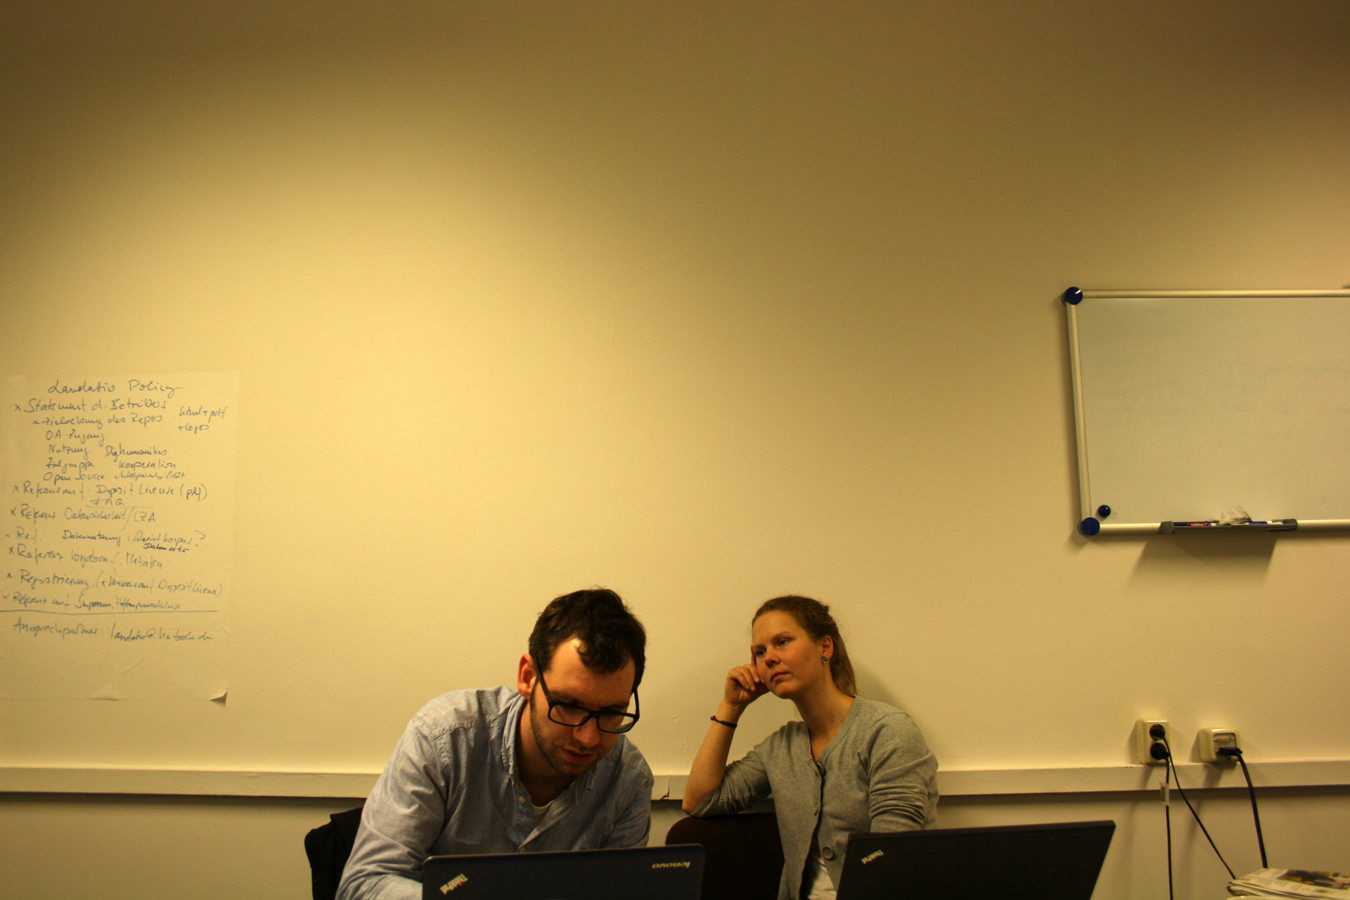
\includegraphics{ediPic.jpg}
\caption{Redaktionsorte V (Berlin-Mitte, März 2014)}
\end{figure}

Die aktuelle Ausgabe der LIBREAS bietet einen kurzen, zeitgenössischen
Einblick in die aktuelle Ausprägung dieser Debattentradition. Die
einzelnen Texte repräsentieren, unserer Meinung nach, sehr schön die
einzelnen Facetten der Diskussion. Begonnen mit einem positiven Aufruf,
die Zukunft gemeinsam mit anderen anzugehen (Corinna Haas und Beate
Rusch); von der Diskussion strukturierter Versuche, zumindest die
nächste Zukunft vorherzusehen (Rudolf Mumenthaler); über einen Rückblick
auf vor teilweise langer Zeit gebaute Zukunftsbibliotheken (Eliane
Blumer \& Karsten Schuldt); bis hin zum nachdrücklichen Hinweis darauf,
dass die Zukunft gestaltet werden muss (Wolfgang Kaiser), stecken die
Texte einen Rahmen ab, in dem sich die meisten Debatten um die
erwünschten, erhofften oder befürchteten Zukünfte der Bibliotheken
bewegen. Dies ersetzt selbstverständlich nicht die weiterhin geführten
Debatten. Aber bereits die zahllosen Beiträge, welche sich in
unterschiedlichen Sprachen nur in den letzten Jahren dieser
Fragestellung befassten, sind kaum vollständig wahrzunehmen. Wobei uns~
Joachim Schöpfel in seinem zum Themenschwerpunkt passenden
Rezensionsbeitrag zeigt, dass diese Debatten nicht nur in Deutsch und
Englisch, sondern zum Beispiel auch sehr tiefgründig in Französisch
geführt werden. Wir hoffen, dass diese Texte wieder einmal Anstöße zu
einer Debatte geben; einer Debatte, die wir auch gerne weiter begleiten
werden.

Dass nicht nur in unserem Metier, sondern auch in der
Literaturwissenschaft Sollbruchstellen existieren, zeigt uns der Text
zur von Joanna Walsh initiierten und bereits vielfach rezipierten Aktion
\#readwomen2014 (Christine Wieder). Wir sind gespannt, was wir in
unserer bereits verkündeten Frauen-Ausgabe -- siehe den
\href{http://libreas.wordpress.com/2013/11/18/4384/}{Call for Papers} im
LIBREAS. Weblog -- über den Fortgang berichten können. Rezensionen zur
nutzerbezogenen Marktforschung (Ulla Wimmer) sowie zu einem in der Reihe
\enquote{Erfolgreich recherchieren} für die Geschichtswissenschaft
erschienenen Bandes (Stefan Wiederkehr), vervollständigen diese Ausgabe.

Egal, in welche Richtung wir persönlich in all den in dieser Ausgabe
aufgeworfenen Fragen tendieren, eines ist uns selbstverständlich allen
klar: The future is unwritten. Und kehrt immer wieder. Insoweit wünschen
wir viele Denkanregungen zu den Zukünften der Bibliotheken, sowohl im
Allgemeinen in der bibliothekarischen Diskussion als auch im Speziellen
in dieser Ausgabe der LIBREAS.

\textbf{Ihre / Eure Redaktion LIBREAS. Library Ideas}

\textbf{(Berlin, Bielefeld, Chur, Mannheim, Potsdam)}

%autor

\end{document}